\documentclass{article}

\usepackage[T1]{fontenc}
\usepackage{graphicx}
\usepackage{fancyhdr}
\pagestyle{fancy}
\fancyhf{}
\lhead{Version 1.0}
\rhead{Elliot Oram}
\rfoot{\thepage}


\title{Overall System Component Diagram}
\author{elo9@aber.ac.uk}

\begin{document}

\maketitle
\tableofcontents

\newpage

\section{Component diagram}
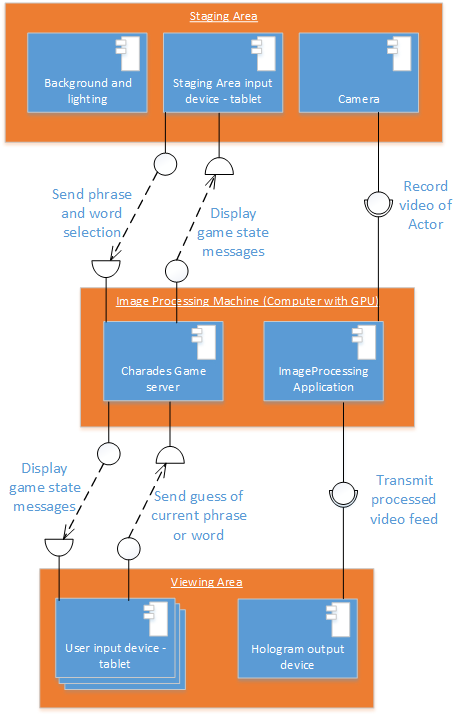
\includegraphics[width=\textwidth]{ComponentDiagramImage}

\newpage


\section{Component diagram description}
\subsection{Staging Area}
The Staging Area details can be found in the Staging Area Design document. The camera directly connects to the ImageProcessing machine via a usb (or similar) cable. The Staging Area input device will use a wireless connection to send and receive messages from the Charades game server that is hosted on the image processing machine.
 
\subsection{Image processing Machine}
The Image Processing machine will be a computer and, due to the nature of the video feed processing in real-time, will require a Graphical processing unit (GPU) - performing spike solutions may be required to ensure that this is the case. The Image Processing application has input of the raw video feed from the camera in the Staging Area and will process the video and output the result.
The Charades Game server is hosted on the Image processing machine. This component will handle the flow between the users in the Viewing Area and the Actor in the Staging Area.

\subsection{Viewing Area}
The Viewing Area will be were the hologram is shown. An output device (A touch screen table being used as an external monitor) will be attached to the Image Processing machine via a HDMI cable. The output device will directly show the result of the ImageProcessing application.
There will be several User input devices in the Viewing Area that will be used to access the Charades Game server.

\end{document}
